% !TeX document-id = {61ff99f0-f133-4544-99cc-74710c877e55}
% !TeX TXS-program:compile = txs:///pdflatex/[--shell-escape]
\documentclass[fleqn,10pt]{beamer}
\usetheme[background=light,titleformat=regular,progressbar=frametitle]{moloch}
\usepackage{amsfonts,amsmath,amssymb,amsthm,booktabs,mathpazo,minted,multicol,optidef,pgfplots,siunitx,sourcecodepro,subcaption,textcomp,thmtools,tikz}
\usepackage[medium]{FiraSans}
\pgfplotsset{compat=1.18}
\usetikzlibrary{shapes,shapes.arrows,arrows.meta,plotmarks,graphs,graphs.standard,calc}
\definecolor{0066cc}{RGB}{0,102,204}
\definecolor{cc0066}{RGB}{204,0,102}
\definecolor{00cc66}{RGB}{0,204,102}
\usemintedstyle{manni}
\definecolor{manni-bg}{RGB}{240,243,243}
\newminted{cpp}{breaklines,frame=lines,linenos,fontsize=\scriptsize,tabsize=4,bgcolor=manni-bg}
\title{Architecture of Modern Finite Element Code}
\subtitle{with an object oriented approach and hybrid parallelisation}
\author{Theodore Chang, Ph.D.}
\date{\today}
\newcount\nodenum
\tikzset{
color0/.style={fill=cc0066!40},
color1/.style={fill=0066cc!40},
setcolor/.code={
\ifnum \nodenum = #1
\global\advance\nodenum 1\relax
\fi
\pgfmathparse{int(mod(\nodenum,2))}
\pgfkeysalso{color\pgfmathresult,node contents=\the\nodenum}
\global\advance\nodenum 1\relax
},
graphs/mygraph/.style={nodes={draw,circle,setcolor=#1,minimum size=4mm},clockwise,radius=#1*.11cm,empty nodes,n=#1},
graphs/mygraph/.append code={\global\nodenum 0\relax}
}
\molochset{block=fill}
\hypersetup{colorlinks}\setbeamercovered{transparent}
\begin{document}
\begin{frame}[plain]
\maketitle
\end{frame}
\section{Objective}
\begin{frame}{Objectives}
\begin{itemize}
\item to report the architecture of \href{https://github.com/TLCFEM/suanPan}{TLCFEM/suanPan}
\begin{itemize}
\item an FEA package written in modern C++ (20)
\item with both shared and distributed memory parallelism
\item covers broad topics in computational solid mechanics
\item contains cutting--edge research outcomes
\item volume: 32k+ tracked lines of code excluding dependencies
\end{itemize}
\item to discuss improvements regarding HPC in simulation
\begin{itemize}
\item parallelisation details
\end{itemize}
\end{itemize}
\end{frame}
\section{Background}
\begin{frame}{Typical FEA Flow}
To analyse a continuum problem with \href{https://www.google.com/search?q=finite+element+method}{FEM}, the following tasks are performed.

\begin{minipage}[b]{.42\linewidth}
\begin{figure}[H]
\centering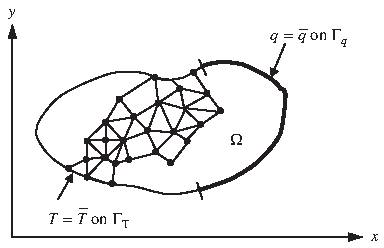
\includegraphics[width=.99\linewidth]{FEM}
\caption*{credit: Fish \& Belytschko, 2007}
\end{figure}
\end{minipage}\hfil
\begin{minipage}[b]{.57\linewidth}
\begin{itemize}
\item discretise the geometry with nodes and elements
\item compute elemental stiffness $\mathbold{K}_e$ and resistance $\mathbold{R}_e$
\item assemble global stiffness $\mathbold{K}=\sum\mathbold{K}_e$ and resistance $\mathbold{R}=\sum\mathbold{R}_e$
\item apply boundary conditions, loads, constraints, etc.
\item solve the system $\mathbold{K}\Delta\mathbold{U}=\mathbold{P}-\mathbold{R}$
\end{itemize}
\end{minipage}
\end{frame}
\begin{frame}{Typical FEA Flow}
\begin{figure}[H]
\centering\scriptsize
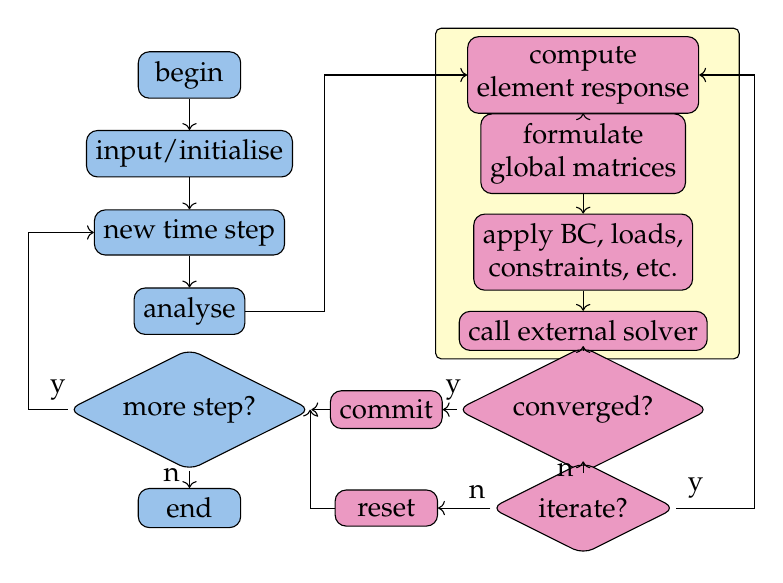
\begin{tikzpicture}
\pgfdeclarelayer{background}
\pgfsetlayers{background,main}
\begin{scope}[every node/.style={rounded corners,draw,fill=0066cc!40,anchor=center,align=center,minimum width=1.3cm,minimum height=4mm}]
\node(begin)at(0,0){begin};
\node(input)at(0,-1){input/initialise};
\node(step)at(0,-2){new time step};
\node(analyse)at(0,-3){analyse};
\node[diamond,aspect=2](more)at(0,-4.25){more step?};
\node(end)at(0,-5.5){end};
\end{scope}
\draw[->](begin.south)--(input.north);
\draw[->](input.south)--(step.north);
\draw[->](step.south)--(analyse.north);
\draw[->](more.south)--(end.north)node[near start,anchor=east]{n};
\draw[->](more.west)--++(-.5,0)node[near start,anchor=south]{y}|-(step.west);
\node at(0,.4){};
\begin{scope}[every node/.style={rounded corners,draw,fill=cc0066!40,anchor=center,align=center,minimum width=1.3cm,minimum height=4mm}]
\node(local)at(5,0){compute\\element response};
\node(global)at(5,-1){formulate\\global matrices};
\node(apply)at(5,-2.25){apply BC, loads,\\constraints, etc.};
\node(solve)at(5,-3.25){call external solver};
\node(converge)[diamond,aspect=2]at(5,-4.25){converged?};
\node(iterate)[diamond,aspect=2]at(5,-5.5){iterate?};
\node(commit)at(2.5,-4.25){commit};
\node(reset)at(2.5,-5.5){reset};
\end{scope}
\draw[->](analyse.east)--++(1,0)|-(local.west);
\draw[->](local.south)--(global.north);
\draw[->](global.south)--(apply.north);
\draw[->](apply.south)--(solve.north);
\draw[->](solve.south)--(converge.north);
\draw[->](converge.west)--(commit.east)node[near start,anchor=south]{y};
\draw[->](commit.west)--(more.east);
\draw[->](converge.south)--(iterate.north)node[near start,anchor=east]{n};
\draw[->](iterate.east)--++(1,0)node[near start,anchor=south]{y}|-(local.east);
\draw[->](iterate.west)--(reset.east)node[near start,anchor=south]{n};
\draw[->](reset.west)-|($(commit.west)-(.25,0)$);
\begin{pgfonlayer}{background}
\draw[rounded corners=2pt,fill=yellow!20]($(local.north west)+(-.4,.1)$)rectangle($(solve.south east)+(.4,-.1)$);
\end{pgfonlayer}
\end{tikzpicture}
\end{figure}
\end{frame}
\section{Storage}
\begin{frame}{Structure}
A complete OO style is used, data are stored in objects arranged in a tree structure.
\begin{figure}[H]
\scriptsize\centering
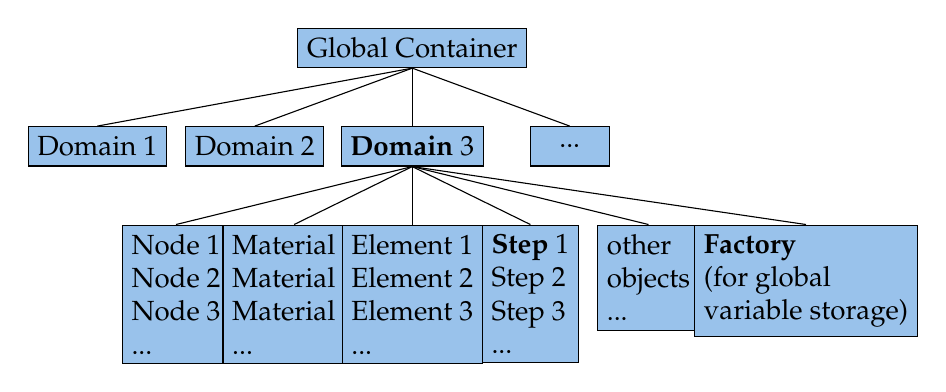
\begin{tikzpicture}[every node/.style={draw,fill=0066cc!40,anchor=north,minimum width=1cm,minimum height=5mm}]
\node(B)at(4,1.25){Global Container};
\node(D1)at(0,0){Domain 1};
\node(D2)at(2,0){Domain 2};
\node(D3)at(4,0){\textbf{Domain} 3};
\node(DN)at(6,0){...};
\node(N)[align=left]at(1,-1.25){Node 1\\Node 2\\Node 3\\...};
\node(M)[align=left]at(2.5,-1.25){Material 1\\Material 2\\Material 3\\...};
\node(E)[align=left]at(4,-1.25){Element 1\\Element 2\\Element 3\\...};
\node(A)[align=left]at(5.5,-1.25){\textbf{Step} 1\\Step 2\\Step 3\\...};
\node(O)[align=left]at(7,-1.25){other\\objects\\...};
\node(F)[align=left]at(9,-1.25){\textbf{Factory}\\(for global\\variable storage)};
\draw(B.south)--(D1.north);
\draw(B.south)--(D2.north);
\draw(B.south)--(D3.north);
\draw(B.south)--(DN.north);
\draw(D3.south)--(N.north);
\draw(D3.south)--(M.north);
\draw(D3.south)--(E.north);
\draw(D3.south)--(A.north);
\draw(D3.south)--(F.north);
\draw(D3.south)--(O.north);
\end{tikzpicture}
\end{figure}
Multiple domains can coexist.
Similar to ABAQUS, multiple analysis steps can be defined in each domain.
Substructuring for distributed memory parallelisation is \underline{theoretically} possible.
\end{frame}
\begin{frame}[containsverbatim]{Domain}
\begin{itemize}
\item represents a problem
\item provides storage for all nodes, elements, materials, integrators, etc.
\end{itemize}
\begin{cppcode}
class Domain {
    shared_ptr<LongFactory> factory; // use double precision

    StepQueue step_pond;

    AmplitudeStorage amplitude_pond;
    ConstraintStorage constraint_pond;
    ElementStorage element_pond;
    MaterialStorage material_pond;
    NodeStorage node_pond;
    SectionStorage section_pond;
    SolverStorage solver_pond;
public:
    // public methods to initialise/update/assemble, etc.
};
\end{cppcode}
\end{frame}
\begin{frame}[containsverbatim]{Storage}
Concurrent containers are used for concurrent insertion/lookup, etc.
Once an object is constructed, no memory reallocation would occur.
Minimum memory operation.
\begin{cppcode}[highlightlines={3}]
template<typename T> class Storage {
    vector<shared_ptr<T>> fish; // some funny variable names
    concurrent_unordered_map<unsigned, shared_ptr<T>, std::hash<unsigned>> pond;
    // ...
};

using AmplitudeStorage = Storage<Amplitude>;
using ConstraintStorage = Storage<Constraint>;
using ElementStorage = Storage<Element>;
using IntegratorStorage = Storage<Integrator>;
// ...
\end{cppcode}
Random access iterator (for easier parallelisation) is provided by \texttt{std::vector<shared\_ptr<T>>}.
\end{frame}
\section{State Updating}
\begin{frame}[standout]
\begin{figure}[H]
\centering\scriptsize
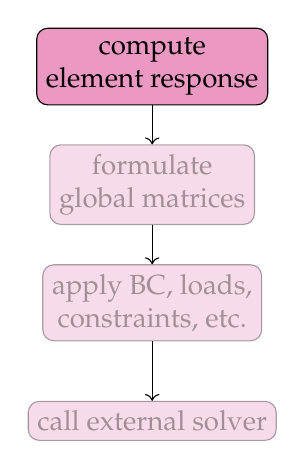
\begin{tikzpicture}
\begin{scope}[every node/.style={rounded corners,draw,fill=cc0066!40,anchor=center,align=center,minimum width=1.3cm,minimum height=4mm}]
\node(local)at(0,0){compute\\element response};
\node[opacity=.35](global)at(0,-1.5){formulate\\global matrices};
\node[opacity=.35](apply)at(0,-3){apply BC, loads,\\constraints, etc.};
\node[opacity=.35](solve)at(0,-4.5){call external solver};
\end{scope}
\draw[->](local.south)--(global.north);
\draw[->](global.south)--(apply.north);
\draw[->](apply.south)--(solve.north);
\end{tikzpicture}
\end{figure}
\end{frame}
\begin{frame}[containsverbatim]{Element Class}
Non-const static variables shall be avoided due to potential racing.
Auxiliary methods can be implemented to hide details.
\begin{cppcode}
class Element : protected DataElement {
protected:
    vector<weak_ptr<Node>> node_ptr; // node pointers

    [[nodiscard]] mat get_coordinate(unsigned) const;

    [[nodiscard]] vec get_incre_displacement() const;
    [[nodiscard]] vec get_trial_displacement() const;
    [[nodiscard]] vec get_current_displacement() const;

    [[nodiscard]] vec get_node_incre_resistance() const;
    [[nodiscard]] vec get_node_trial_resistance() const;
    [[nodiscard]] vec get_node_current_resistance() const;
public:
    // ...
};
\end{cppcode}
\end{frame}
\begin{frame}[containsverbatim]{Element Class}
A general purpose dataset is provided to manage state internally.
There is no interaction with the outside.
\begin{cppcode}
struct DataElement {
    const uvec node_encoding; // node encoding
    const uvec material_tag;  // material tags

    mat initial_mass{}; // mass matrix
    mat trial_mass{};   // mass matrix
    mat current_mass{}; // mass matrix

    mat initial_stiffness{}; // stiffness matrix
    mat trial_stiffness{};   // stiffness matrix
    mat current_stiffness{}; // stiffness matrix

    vec trial_resistance{};            // resistance vector
    vec current_resistance{};          // resistance vector
    // ...
};
\end{cppcode}
\end{frame}
\begin{frame}[containsverbatim]{Element Class}
$\mathbold{K}_e=\sum\mathbold{B}^\mathrm{T}\mathbold{E}\mathbold{B}$. Expressive code with high performing lazy evaluation.
\begin{cppcode}[fontsize=\tiny,highlightlines={18-20}]
// header
class C3D20 final : public MaterialElement3D {
    struct IntegrationPoint final {
        double weight;
        unique_ptr<Material> c_material;
        mat strain_mat;
    };
    // ...
    vector<IntegrationPoint> int_pt;
};

// implementation
int C3D20::update_status() {
    trial_stiffness.zeros(c_size, c_size);
    trial_resistance.zeros(c_size);

    for(const auto& I : int_pt) {
        I.c_material->update_trial_status(I.strain_mat * get_trial_displacement());
        trial_stiffness += I.weight * I.strain_mat.t() * I.c_material->get_trial_stiffness() * I.strain_mat;
        trial_resistance += I.weight * I.strain_mat.t() * I.c_material->get_trial_stress();
    }

    return SUANPAN_SUCCESS;
}
\end{cppcode}
\end{frame}
\begin{frame}[containsverbatim]{Material Class}
Similar to \texttt{Element}, if pre-defined dataset is used, state is managed internally and automatically.

Only need to provide the method to compute stress $\mathbold{\sigma}$ and stiffness $\mathbold{E}$ for given strain $\mathbold{\varepsilon}$. No external data dependency. Similar to the UMAT subroutine in ABAQUS.

For linear elastic response, $\mathbold{\sigma=E\varepsilon}$.
\begin{cppcode}
int Elastic1D::update_trial_status(const vec& t_strain) {
    trial_strain = t_strain;
    trial_stiffness = elastic_modulus;
    trial_stress = trial_stiffness * trial_strain;
    return SUANPAN_SUCCESS;
}
\end{cppcode}
\end{frame}
\begin{frame}{State Updating}
Each element manages its state independently and updates its state based on global nodal displacement vector.
\begin{gather*}
\mathbold{U}\Longrightarrow\mathbold{\varepsilon}_e\Longrightarrow\mathbold{\sigma}_e\Longrightarrow\mathbold{K}_e,~\mathbold{R}_e
\end{gather*}
concurrent-read-no-write, no racing, lock free, can be safely parallelised
\begin{figure}[H]
\scriptsize\centering
\begin{tikzpicture}
\pgfdeclarelayer{background}
\pgfsetlayers{background,main}
\begin{scope}[every node/.style={draw,fill=black!20,anchor=north,minimum width=1.5cm,minimum height=5mm}]
\node(B)at(4,2.5){Domain};
\node(E1)at(0,0){Element 1};
\node(E2)at(2,0){Element 2};
\node(E3)at(4,0){Element 3};
\node(E4)at(6,0){Element 4};
\node(E5)at(8,0){...};
\draw[->](B.south)--++(0,-1)-|(E1.north);
\draw[->](B.south)--++(0,-1)-|(E2.north);
\draw[->](B.south)--(E3.north);
\draw[->](B.south)--++(0,-1)-|(E4.north);
\draw[->](B.south)--++(0,-1)-|(E5.north);
\end{scope}
\node[fill=bg]at($(B.south)+(0,-.6)$){\texttt{Domain::update\_status()}};
\begin{pgfonlayer}{background}
\path(B.north -| E1.west)+(-.2,.5)node(a){};
\path(B.south -| E5.east)+(.2,-.25)node(b){};
\path(E1.north west)+(-.2,.5)node(c){};
\path(E2.south east)+(.2,-.25)node(d){};
\path(E3.north west)+(-.2,.5)node(e){};
\path(E4.south east)+(.2,-.25)node(f){};
\path(E5.north west)+(-.2,.5)node(g){};
\path(E5.south east)+(.2,-.25)node(h){};
\draw[rounded corners=2pt,fill=cc0066!20](a)node[anchor=north west]{dispatcher}rectangle(b);
\draw[rounded corners=2pt,fill=0066cc!20](c)node[anchor=north west]{worker}rectangle(d);
\draw[rounded corners=2pt,fill=0066cc!20](e)node[anchor=north west]{worker}rectangle(f);
\draw[rounded corners=2pt,fill=0066cc!20](g)node[anchor=north west]{worker}rectangle(h);
\end{pgfonlayer}
\end{tikzpicture}
\end{figure}
\end{frame}
\begin{frame}[containsverbatim]{State Updating}
Optimal performance is achieved through hybrid parallelism.
Each compute node manages a specific subset of elements, updating them concurrently via shared memory without the need for message passing.
\begin{cppcode}[highlightlines={5}]
int Domain::update_trial_status() const {
    suanpan::for_all(node_pond.get(), [&](const shared_ptr<Node>& t_node) { t_node->update_trial_status(trial_displacement, trial_velocity, trial_acceleration); });

    suanpan::for_all(element_pond.get(), [&](const shared_ptr<Element>& t_element) {
        if(t_element->is_local) t_element->update_status();
    });
    // ...
}
\end{cppcode}
\end{frame}
\section{Global Assembly}
\begin{frame}[standout]
\begin{figure}[H]
\centering\scriptsize
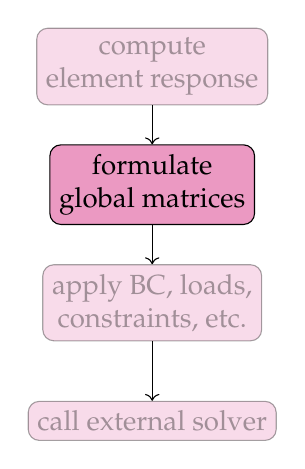
\begin{tikzpicture}
\begin{scope}[every node/.style={rounded corners,draw,fill=cc0066!40,anchor=center,align=center,minimum width=1.3cm,minimum height=4mm}]
\node[opacity=.35](local)at(0,0){compute\\element response};
\node(global)at(0,-1.5){formulate\\global matrices};
\node[opacity=.35](apply)at(0,-3){apply BC, loads,\\constraints, etc.};
\node[opacity=.35](solve)at(0,-4.5){call external solver};
\end{scope}
\draw[->](local.south)--(global.north);
\draw[->](global.south)--(apply.north);
\draw[->](apply.south)--(solve.north);
\end{tikzpicture}
\end{figure}
\end{frame}
\begin{frame}{Global Matrix Assembly}
Assembling elemental stiffness $\mathbold{K}_e$ into global stiffness $\mathbold{K}$ is often done sequentially due to data overlapping.

Mutex may be expensive. Instead, the reliable $k$-coloring algorithm can be used. The earliest reference dates back to 1982.
\begin{figure}[H]
\centering\scriptsize
\definecolor{mycolor1}{rgb}{0.00000,0.44700,0.74100}
\begin{tikzpicture}
\begin{axis}[
width=1.5in,
height=1.5in,
scale only axis,
xmin=0,
xmax=11,
y dir=reverse,
ymin=0,
ymax=11,
hide axis,
xtick=\empty,
ytick=\empty
]
\addplot[color=mycolor1, draw=none, mark size=2.3pt, mark=*, mark options={solid, mycolor1}]
table[row sep=crcr]{
1	1\\
1	2\\
2	1\\
2	2\\
2	3\\
3	2\\
3	3\\
3	4\\
4	3\\
4	4\\
4	5\\
5	4\\
5	5\\
5	6\\
6	5\\
6	6\\
6	7\\
7	6\\
7	7\\
7	8\\
8	7\\
8	8\\
8	9\\
9	8\\
9	9\\
9	10\\
10	9\\
10	10\\
};
\draw(axis cs:.5,.5)rectangle(axis cs:10.5,10.5);
\draw(axis cs:1.5,3.5)rectangle(axis cs:3.5,1.5)node[right=1mm]{$\mathbold{K}_e^2$};
\draw(axis cs:2.5,4.5)rectangle(axis cs:4.5,2.5)node[right=1mm]{$\mathbold{K}_e^3$};
\end{axis}
\end{tikzpicture}
\hfil
\input{SPY2}
\end{figure}
\end{frame}
\begin{frame}[containsverbatim]{Global Matrix Assembly}
\begin{minipage}{.64\textwidth}
\begin{itemize}
\item initialisation
\begin{enumerate}
\item construct the graph
\item color the graph
\item store the coloring scheme
\end{enumerate}
\item state updating
\begin{enumerate}
\item loop over all color groups
\item update all elements in the same group
\end{enumerate}
\end{itemize}
\end{minipage}\hfil
\begin{minipage}{.35\textwidth}
\centering\tiny
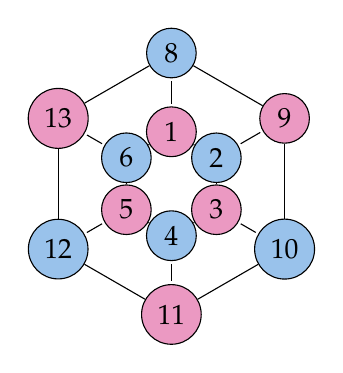
\begin{tikzpicture}
\graph[mygraph=6]{
subgraph C_n[name=inner]--[shorten <=1pt,shorten >=1pt]
subgraph C_n[name=outer]
};
\end{tikzpicture}
\end{minipage}

\begin{cppcode}[fontsize=\tiny]
void Domain::assemble_trial_stiffness() const {
    std::ranges::for_each(color_map, [&](const std::vector<unsigned>& color) {
        suanpan::for_all(color, [&](const unsigned tag) {
            if(const auto& I = get_element(tag); I->is_local) factory->assemble_stiffness(I->get_trial_stiffness(), I->get_dof_encoding(), I->get_dof_mapping());
        });
    });

    factory->get_stiffness()->allreduce();
}
\end{cppcode}
\end{frame}
\begin{frame}{Global Matrix Assembly}
Pre-coloring the model leads to a \textbf{lock-free} algorithm for \textbf{parallel} matrix assembly with the \textbf{dense} storage.

What about the \textbf{sparse} storage?
Use COO format and pre-allocate memory blocks, $\mathbold{K}_e$ can be copied into $\mathbold{K}$ in parallel.
Since $\mathbold{K}_e$ spans contiguous memory, the copy operation may be automatically vectorised by compiler via SIMD.

Elemental quantities are assembled locally on each compute node to formulate the partial global matrices/vectors.
Only these partial quantities will be reduced (synchronised) to formulate the final full quantities.
\end{frame}
%\begin{frame}[containsverbatim]{Distributed Approach A--- Scattering}
%A process ID is assigned to each element, in the following, elements 1 and 3 are assigned to the root process, elements 2 and 4 are assigned to the other process.
%When \texttt{update\_status()} is called, each process updates the elements assigned to itself, and skips all other elements.
%\begin{figure}[H]
%\scriptsize\centering
%\begin{tikzpicture}
%\pgfdeclarelayer{background}
%\pgfsetlayers{background,main}
%\begin{scope}[every node/.style={draw,fill=black!20,anchor=north,minimum width=1.5cm,minimum height=5mm}]
%\node(B)at(1,2){Domain};
%\node(E1)at(0,0){Element 1};
%\node[dashed,fill=black!10](E2)at(2,0){Element 2};
%\node(E3)at(0,-1){Element 3};
%\node[dashed,fill=black!10](E4)at(2,-1){Element 4};
%\draw[->](B.south)--++(0,-1);
%\end{scope}
%\node[fill=bg]at($(B.south)+(0,-.6)$){\texttt{update\_status()}};
%\begin{pgfonlayer}{background}
%\path(B.north -| E1.west)+(-.2,.5)node(a){};
%\path(B.south -| E4.east)+(.2,-.25)node(b){};
%\path(E1.north west)+(-.2,.5)node(c){};
%\path(E4.south east)+(.2,-.2)node(f){};
%\draw[rounded corners=2pt,fill=cc0066!20](a)node[anchor=north west]{root process}rectangle(b);
%\draw[rounded corners=2pt,fill=0066cc!20](c)rectangle(f);
%\end{pgfonlayer}
%\begin{scope}[xshift=6cm]
%\begin{scope}[every node/.style={draw,fill=black!20,anchor=north,minimum width=1.5cm,minimum height=5mm}]
%\node(B)at(1,2){Domain};
%\node[dashed,fill=black!10](E1)at(0,0){Element 1};
%\node(E2)at(2,0){Element 2};
%\node[dashed,fill=black!10](E3)at(0,-1){Element 3};
%\node(E4)at(2,-1){Element 4};
%\draw[->](B.south)--++(0,-1);
%\end{scope}
%\node[fill=bg]at($(B.south)+(0,-.6)$){\texttt{update\_status()}};
%\begin{pgfonlayer}{background}
%\path(B.north -| E1.west)+(-.2,.5)node(a){};
%\path(B.south -| E4.east)+(.2,-.25)node(b){};
%\path(E1.north west)+(-.2,.5)node(c){};
%\path(E4.south east)+(.2,-.2)node(f){};
%\draw[rounded corners=2pt,fill=cc0066!20](a)node[anchor=north west]{the other process}rectangle(b);
%\draw[rounded corners=2pt,fill=0066cc!20](c)rectangle(f);
%\end{pgfonlayer}
%\end{scope}
%\end{tikzpicture}
%\end{figure}
%\end{frame}
%\begin{frame}[containsverbatim]{Distributed Approach A --- Gathering}
%To collect elemental resistance/stiffness, all other processes send data to the root process.
%By the end of this communication, the root process contains all elemental quantities stored in local objects.
%They hold the final results, which may not be computed by themselves (sent over from remote objects).
%\begin{figure}[H]
%\scriptsize\centering
%\begin{tikzpicture}
%\pgfdeclarelayer{background}
%\pgfsetlayers{background,main}
%\begin{scope}[every node/.style={draw,fill=black!20,anchor=north,minimum width=1.5cm,minimum height=5mm}]
%\node(B)at(1,2){Domain};
%\node(E1)at(0,0){Element 1};
%\node(E2)at(2,0){Element 2};
%\node(E3)at(0,-1){Element 3};
%\node(E4)at(2,-1){Element 4};
%\draw[->](B.south)--++(0,-1);
%\end{scope}
%\node[fill=bg]at($(B.south)+(0,-.6)$){\texttt{assemble\_trial\_stiffness()}};
%\begin{pgfonlayer}{background}
%\path(B.north -| E1.west)+(-.2,.5)node(a){};
%\path(B.south -| E4.east)+(.2,-.25)node(b){};
%\path(E1.north west)+(-.2,.5)node(c){};
%\path(E4.south east)+(.2,-.2)node(f){};
%\draw[rounded corners=2pt,fill=cc0066!20](a)node[anchor=north west]{root process}rectangle(b);
%\draw[rounded corners=2pt,fill=0066cc!20](c)rectangle(f);
%\end{pgfonlayer}
%\begin{scope}[xshift=6cm]
%\begin{scope}[every node/.style={draw,fill=black!20,anchor=north,minimum width=1.5cm,minimum height=5mm}]
%\node(B)at(1,2){Domain};
%\node[dashed,fill=black!10](E1)at(0,0){Element 1};
%\node(E2)at(2,0){Element 2};
%\node[dashed,fill=black!10](E3)at(0,-1){Element 3};
%\node(E4)at(2,-1){Element 4};
%\draw[->](B.south)--++(0,-1);
%\end{scope}
%\node[fill=bg]at($(B.south)+(0,-.6)$){\texttt{assemble\_trial\_stiffness()}};
%\begin{pgfonlayer}{background}
%\path(B.north -| E1.west)+(-.2,.5)node(a){};
%\path(B.south -| E4.east)+(.2,-.25)node(b){};
%\path(E1.north west)+(-.2,.5)node(c){};
%\path(E4.south east)+(.2,-.2)node(f){};
%\draw[rounded corners=2pt,fill=cc0066!20](a)node[anchor=north west]{the other process}rectangle(b);
%\draw[rounded corners=2pt,fill=0066cc!20](c)rectangle(f);
%\end{pgfonlayer}
%\draw[->](E2.north)--++(0,.2)--++(-6,0)node[pos=.65,anchor=center,fill=bg]{\texttt{send/recv}}--++(0,-.2);
%\draw[->](E4.north)--++(0,.2)--++(-6,0)node[pos=.65,anchor=center,fill=bg]{\texttt{send/recv}}--++(0,-.2);
%\end{scope}
%\end{tikzpicture}
%\end{figure}
%\end{frame}
%\begin{frame}[containsverbatim]{Distributed Approach A --- Traits}
%\begin{itemize}
%\item relatively large memory footprint on each node
%\item minimal data transfer
%\item no temporary memory (de)allocation
%\item no (de)serialisation of objects
%\item simple P2P communication pattern (only \texttt{bcast}, \texttt{send}, \texttt{recv})
%\item \bfseries\color{cc0066}a large number (proportional to the number of elements) of small messages
%\end{itemize}
%\end{frame}
\begin{frame}[containsverbatim]{Distributed Approach --- Gathering}
\begin{figure}[H]
\scriptsize\centering
\begin{tikzpicture}
\pgfdeclarelayer{background}
\pgfsetlayers{background,main}
\begin{scope}[every node/.style={draw,fill=black!20,anchor=north,minimum width=1.5cm,minimum height=5mm}]
\node(B)at(1,1.8){Domain};
\coordinate(E1)at(-.5,.3);
\coordinate(E2)at(2.5,-2);
\draw[fill=black!20](E1)rectangle(E2)node[anchor=center,midway,align=center]{partial global stiffness\\$\begin{bmatrix}
*&*&\cdot&\cdot\\
*&*&\cdot&\cdot\\
\cdot&\cdot&\cdot&\cdot\\
\cdot&\cdot&\cdot&\cdot
\end{bmatrix}$};
\draw[->](B.south)--++(0,-1);
\end{scope}
\node[fill=bg]at($(B.south)+(0,-.5)$){\texttt{assemble\_trial\_stiffness()}};
\begin{pgfonlayer}{background}
\path(B.north -| E1.west)+(-.2,.4)node(a){};
\path(B.south -| E2.east)+(.2,-.2)node(b){};
\path(E1.north west)+(-.2,.2)node(c){};
\path(E2.south east)+(.2,-.2)node(f){};
\draw[rounded corners=2pt,fill=cc0066!20](a)node[anchor=north west]{root process/node}rectangle(b);
\draw[rounded corners=2pt,fill=0066cc!20](c)rectangle(f);
\end{pgfonlayer}
\begin{scope}[xshift=6cm]
\begin{scope}[every node/.style={draw,fill=black!20,anchor=north,minimum width=1.5cm,minimum height=5mm}]
\node(B)at(1,1.8){Domain};
\coordinate(E1)at(-.5,.3);
\coordinate(E2)at(2.5,-2);
\draw[fill=black!20](E1)rectangle(E2)node[anchor=center,midway,align=center]{partial global stiffness\\$\begin{bmatrix}
\cdot&\cdot&\cdot&\cdot\\
\cdot&*&*&*\\
\cdot&*&*&*\\
\cdot&*&*&*
\end{bmatrix}$};
\draw[->](B.south)--++(0,-1);
\end{scope}
\node[fill=bg]at($(B.south)+(0,-.5)$){\texttt{assemble\_trial\_stiffness()}};
\begin{pgfonlayer}{background}
\path(B.north -| E1.west)+(-.2,.4)node(a){};
\path(B.south -| E2.east)+(.2,-.2)node(b){};
\path(E1.north west)+(-.2,.2)node(c){};
\path(E2.south east)+(.2,-.2)node(f){};
\draw[rounded corners=2pt,fill=cc0066!20](a)node[anchor=north west]{the other process/node}rectangle(b);
\draw[rounded corners=2pt,fill=0066cc!20](c)rectangle(f);
\end{pgfonlayer}
\draw[->](-2,-1)--++(0,-1);
\draw[-](-.5,-1)--++(-3,0)node[pos=.5,anchor=center,fill=bg,align=center]{\texttt{reduce}\\\texttt{allreduce}};
\end{scope}
\node[fill=black!20,anchor=north,align=center]at(4,-2){global stiffness\\$\begin{bmatrix}
*&*&\cdot&\cdot\\
*&*&*&*\\
\cdot&*&*&*\\
\cdot&*&*&*
\end{bmatrix}$};
\end{tikzpicture}
\end{figure}
\end{frame}
\begin{frame}[containsverbatim]{Distributed Approach --- Traits}
\begin{itemize}
\item relatively large memory footprint on each compute node
\item no (de)serialisation (messaging passing) of (small) objects
\item no temporary memory (de)allocation
\item simple collective communication pattern (only \texttt{bcast}, \texttt{reduce}/\texttt{allreduce})
\item \bfseries\color{cc0066}minimal number (proportional to the number of processes) of large messages, less concerning because latency matters
\end{itemize}
\end{frame}
\begin{frame}[standout]
\begin{figure}[H]
\centering\scriptsize
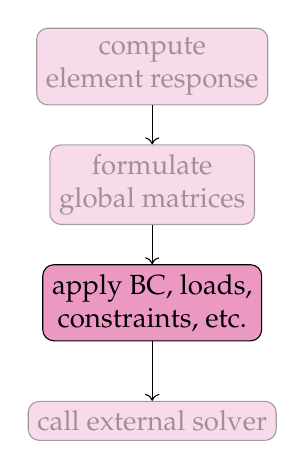
\begin{tikzpicture}
\begin{scope}[every node/.style={rounded corners,draw,fill=cc0066!40,anchor=center,align=center,minimum width=1.3cm,minimum height=4mm}]
\node[opacity=.35](local)at(0,0){compute\\element response};
\node[opacity=.35](global)at(0,-1.5){formulate\\global matrices};
\node(apply)at(0,-3){apply BC, loads,\\constraints, etc.};
\node[opacity=.35](solve)at(0,-4.5){call external solver};
\end{scope}
\draw[->](local.south)--(global.north);
\draw[->](global.south)--(apply.north);
\draw[->](apply.south)--(solve.north);
\end{tikzpicture}
\end{figure}
\end{frame}
\begin{frame}{Loads and Constraints}
Consider the optimisation problem:
\begin{mini*}|l|
{}{W\left(\mathbold{u}\right)}
{}{}
\addConstraint{\mathbold{c\left(u\right)=0}}
\end{mini*}
In which $W$ is the strain energy function, $\mathbold{c}$ contains $n$ constraints.

The Lagrange function can be constructed as
\begin{gather*}
\mathcal{L}\left(\mathbold{u},~\mathbold{\lambda}\right)=W\left(\mathbold{u}\right)+\mathbold{\lambda}\cdot\mathbold{c\left(u\right)}.
\end{gather*}
The stationary point can be obtained
\begin{gather*}
\nabla\mathcal{L}\left(\mathbold{u},~\mathbold{\lambda}\right)=\mathbold{0},\qquad\longrightarrow\qquad\left\{\begin{array}{l}
\mathbold{R}+\mathbold{\lambda}\cdot\nabla\mathbold{c}=\mathbold{0},\\
\mathbold{c}=\mathbold{0}.
\end{array}\right.
\end{gather*}
In which $\mathbold{R}=\nabla{}W$ is the resistance.
\end{frame}
\begin{frame}{Loads and Constraints}
Consider a nonlinear context, the system shall be iteratively solved. The effective stiffness is then
\begin{gather*}
\mathbold{J}=\begin{bmatrix}
\mathbold{K}&\cdot\\
\cdot&\cdot
\end{bmatrix}+
\begin{bmatrix}
\nabla^2\mathbold{c}&\nabla\mathbold{c}^\mathrm{T}\\
\nabla\mathbold{c}&\cdot
\end{bmatrix}=\begin{bmatrix}
\mathbold{K}+\mathbold{K}_c&\mathbold{K}_b^\mathrm{T}\\
\mathbold{K}_b&\cdot
\end{bmatrix}
\end{gather*}
$\mathbold{K}_b$ is known as border matrix. Often, it is \textbf{sparse}. The size of global stiffness changes due to the presence of constraints.

Since the number of constraints is not known in advance, memory reallocation is required, which is not preferred.

Noting $\mathbold{K}_c$ is similar to elemental stiffness $\mathbold{K}_e$ and can be assembled into $\mathbold{K}$, it is possible to store $\mathbold{K}_b$ separately and static condensation can be used to solve the system. The additional cost is only forward/backward substitution as $\mathbold{K}+\mathbold{K}_c$ should have been factorised.
\end{frame}
\begin{frame}[containsverbatim]{Loads and Constraints}
Constraints can be updated and assembled concurrently. The same constraint can have different number of multipliers during different phases of analysis. Loads can be handled in the same manner.
\begin{cppcode}
// ...
auto counter = 0;
for(auto& I : constraint_pond.get()) {
    const auto m_size = I->get_multiplier_size();
    if(!I->is_initialized() || 0 == m_size) continue;
    const auto e_size = counter + m_size - 1;
    t_resistance.subvec(counter, e_size) = I->get_auxiliary_resistance();
    t_load.subvec(counter, e_size) = I->get_auxiliary_load();
    t_stiffness.cols(counter, e_size) = I->get_auxiliary_stiffness();
    counter += m_size;
}
// ...
\end{cppcode}
\end{frame}
\section{Solving}
\begin{frame}[standout]
\begin{figure}[H]
\centering\scriptsize
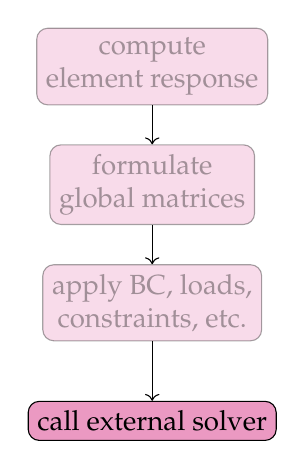
\begin{tikzpicture}
\begin{scope}[every node/.style={rounded corners,draw,fill=cc0066!40,anchor=center,align=center,minimum width=1.3cm,minimum height=4mm}]
\node[opacity=.35](local)at(0,0){compute\\element response};
\node[opacity=.35](global)at(0,-1.5){formulate\\global matrices};
\node[opacity=.35](apply)at(0,-3){apply BC, loads,\\constraints, etc.};
\node(solve)at(0,-4.5){call external solver};
\end{scope}
\draw[->](local.south)--(global.north);
\draw[->](global.south)--(apply.north);
\draw[->](apply.south)--(solve.north);
\end{tikzpicture}
\end{figure}
\end{frame}
\begin{frame}[containsverbatim]{Analysis Logic}
Multiple steps can be defined, they'll be analysed sequentially.
\begin{cppcode}[fontsize=\tiny]
for(const auto& t_domain : domain_pool)
    if(t_domain->is_active())
        for(const auto& t_step : t_domain->get_step_pool()) {
            // ...
            if(SUANPAN_FAIL == t_step->Step::initialize()) return SUANPAN_FAIL;
            if(SUANPAN_FAIL == t_step->initialize()) return SUANPAN_FAIL;
            if(SUANPAN_FAIL == t_step->analyze()) return SUANPAN_FAIL;
        }
\end{cppcode}
\begin{figure}[H]
\scriptsize\centering
\begin{tikzpicture}
\begin{scope}[every node/.style={draw,fill=0066cc!40,anchor=center,minimum width=1.3cm,minimum height=4mm}]
\node(S)at(0,0){Step};
\node(SV)at(2,0){Solver};
\node(I)at(4.5,0){Integrator};
\node(D)at(7,0){Domain};
\node(N)at(9,0){Node};
\node(E)at(9,-.7){Element};
\node(C)at(9,-1.4){Constraint};
\node(M)at(9,-2.1){...};
\node(F)at(4.5,-2){Factory};
\draw[->](D.east)--++(.3,0)|-(E.west);
\draw[->](D.east)--++(.3,0)|-(C.west);
\draw[->](D.east)--++(.3,0)|-(M.west);
\end{scope}
\begin{tiny}
\draw[->](D.east)--(N.west)node[midway,above=3mm,align=center]{manage state};
\draw[->](S.east)--(SV.west)node[midway,above=3mm,align=center]{manage convergence,\\time marching, etc.};
\draw[->](SV.east)--(I.west)node[midway,above=3mm,align=center]{formulate, solve system\\via external solver};
\draw[->](I.east)--(D.west)node[midway,above=3mm,align=center]{wrapper};
\draw[->](I.south)--(F.north)node[midway,align=center,fill=bg]{modify to consider\\global damping, etc.};
\draw[->](F.west)-|(SV.south)node[near start,align=center]{return new trial\\displacement};
\draw[->](D.south)|-(F.east)node[near end,align=center]{assemble\\global vec/mat};
\end{tiny}
\end{tikzpicture}
\end{figure}
\end{frame}
\begin{frame}{Analysis Logic}
\begin{figure}[H]
\scriptsize\centering
\begin{tikzpicture}
\begin{scope}[every node/.style={draw,fill=0066cc!40,anchor=center,minimum width=1.3cm,minimum height=4mm}]
\node(S)at(0,0){Step};
\node(SV)at(2,0){Solver};
\node(I)at(4.5,0){\color{cc0066}Integrator};
\node(D)at(7,0){Domain};
\node(N)at(9,0){Node};
\node(E)at(9,-.7){Element};
\node(C)at(9,-1.4){Constraint};
\node(M)at(9,-2.1){...};
\node(F)at(4.5,-2){Factory};
\draw[->](D.east)--++(.3,0)|-(E.west);
\draw[->](D.east)--++(.3,0)|-(C.west);
\draw[->](D.east)--++(.3,0)|-(M.west);
\end{scope}
\begin{tiny}
\draw[->](D.east)--(N.west)node[midway,above=3mm,align=center]{manage state};
\draw[->](S.east)--(SV.west)node[midway,above=3mm,align=center]{manage convergence,\\time marching, etc.};
\draw[->](SV.east)--(I.west)node[midway,above=3mm,align=center]{formulate, solve system\\via external solver};
\draw[->](I.east)--(D.west)node[midway,above=3mm,align=center]{wrapper};
\draw[->](I.south)--(F.north)node[midway,align=center,fill=bg]{modify to consider\\global damping, etc.};
\draw[->](F.west)-|(SV.south)node[near start,align=center]{return new trial\\displacement};
\draw[->](D.south)|-(F.east)node[near end,align=center]{assemble\\global vec/mat};
\end{tiny}
\end{tikzpicture}
\end{figure}
\begin{itemize}
\item \texttt{Solver} does not directly communicate with data storage \texttt{Domain} and \texttt{Factory}
\item \texttt{Factory} does not directly communicate with local data storage \texttt{Element}, etc.
\item Different operations can be injected via overloading.
\end{itemize}
\end{frame}
\begin{frame}[containsverbatim]{System Solving}
\texttt{Solver} implements different solving algorithms such as (modified) Newton, BFGS, displacement control, arc length control, etc.
\begin{cppcode}
int Newton::analyze() {
    // ...
    // G is an Integrator
    while(true) {
        G->assemble_resistance(); // in parallel
        G->assemble_matrix();     // in parallel
        G->process_load();        // in parallel
        G->process_constraint();  // in parallel

        G->solve(ninja, G->get_force_residual()); // X=inv(A)*B

        G->update_trial_displacement(ninja); // sync global in parallel
        G->update_trial_status();            // sync local in parallel

        if(C->is_converged()) return SUANPAN_SUCCESS; // exit if converged
        if(++counter > max_iteration) return SUANPAN_FAIL;
    }
}
\end{cppcode}
\end{frame}
\begin{frame}[containsverbatim]{Analysis Type}
Basic utility methods in \texttt{Domain} can be invoked in parallel on demand to fulfil the desired task.
\begin{gather*}
\bar{\mathbold{K}}=\mathbold{K}+c_0\mathbold{M}+c_1\mathbold{C}
\end{gather*}
\begin{cppcode}
// Newmark is derived from Integrator
void Newmark::assemble_matrix() {
    const auto& D = get_domain().lock(); // weak_ptr
    auto& W = D->get_factory();

    D->assemble_trial_stiffness();
    D->assemble_trial_mass();
    D->assemble_trial_damping();

    // this addition is also parallelised
    W->get_stiffness() += C0 * W->get_mass() + C1 * W->get_damping();
}
\end{cppcode}
\end{frame}
\begin{frame}{Matrix Storage Scheme}
\begin{itemize}
\item in-house matrix container that supports:
\begin{itemize}
\item dense (full, banded, symm./asymm.)
\item sparse (COO, CSC, CSR)
\end{itemize}
\item fully decoupled from the FE model
\item easy to add new solvers, override \texttt{MetaMat::solve()} method
\item both double and mixed precision solving strategy
\item currently available:
\begin{multicols}{2}
\begin{itemize}
\item OpenBLAS
\item MKL
\item SPIKE
\item ARPACK
\item FEAST
\item SuperLU
\item MUMPS
\item CUDA
\end{itemize}
\end{multicols}
\item distributed memory model based solvers are managed independently
\end{itemize}
\end{frame}
\begin{frame}[containsverbatim]{Distributed Solvers}
\href{https://github.com/TLCFEM/ezp}{TLCFEM/ezp}: lightweight C++ wrapper for distributed solvers

With roughly 2k lines of code, it manages to:
\begin{itemize}
\item hides all MPI details
\item hides all solver details
\item exposes an interface similar to the sequential counterpart
\item requires zero extra setup --- the global matrix collected from the previous step can be directly passed in and solved
\end{itemize}
\end{frame}
\begin{frame}[containsverbatim]{Distributed Solvers --- Example}
\begin{cppcode}[fontsize=\tiny,highlightlines={13-17,20}]
#include <ezp/pgesv.hpp>
#include <iomanip>
#include <iostream>

using namespace ezp;

int main() {
    const auto rank = get_env<int>().rank();
    constexpr auto N = 6, NRHS = 2;
    std::vector<double> A, B;

    if(0 == rank) {
        A.resize(N * N, 0.);
        B.resize(N * NRHS, 1.);

        const auto IDX = par_dgesv<int>::indexer{N};
        for(auto I = 0; I < N; ++I) A[IDX(I, I)] = static_cast<double>(I);
    }

    par_dgesv<int>().solve({N, N, A.data()}, {N, NRHS, B.data()});

    if(0 == rank) {
        std::cout << std::setprecision(10) << "Solution:\n";
        for(auto i = 0; i < B.size(); ++i) std::cout << B[i] << '\n';
    }

    return 0;
}
\end{cppcode}
\end{frame}
\section{Benchmark}
\begin{frame}{Benchmark}
\begin{minipage}{.54\textwidth}
\begin{itemize}
\item i7-8700 (6C12T) with DDR4-2666
\item about 120 GFLOPS (pure DGEMM)
\item 120744 DoFs
\item 39990 three-node shell elements
\item linear elastic material
\item 40 complete analysis cycles
\item solved by DPBSV
\end{itemize}
\end{minipage}
\begin{minipage}{.45\textwidth}
\centering
\includegraphics[width=.99\textwidth]{DKTS3}
\end{minipage}
\end{frame}
\begin{frame}{Benchmark}
with default MKL configurations
\begin{itemize}
\item \numrange{105}{107} GFLOPS overall
\item additional \num{10} GFLOPS excluding initialisation
\item \SI{80}{\percent} CPU utilisation
\end{itemize}
\begin{figure}[H]
\centering
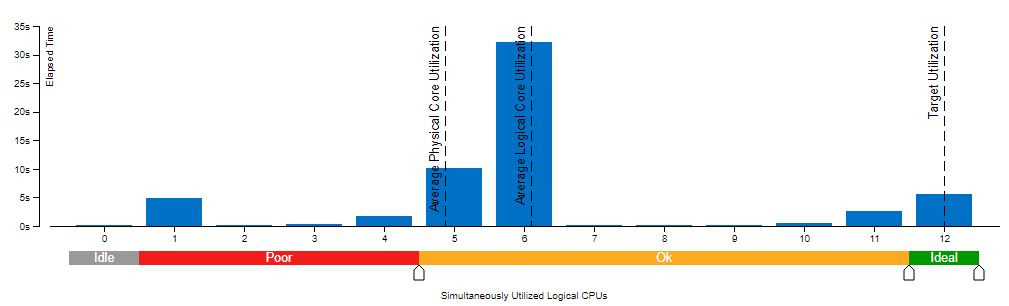
\includegraphics[width=.99\linewidth]{B2}
\end{figure}
\end{frame}
\begin{frame}{Benchmark}
with default MKL configurations
\begin{itemize}
\item \SI{80}{\percent} CPU utilisation
\item \numrange{105}{107} GFLOPS overall
\item additional \num{10} GFLOPS excluding initialisation
\end{itemize}
\begin{figure}[H]
\centering
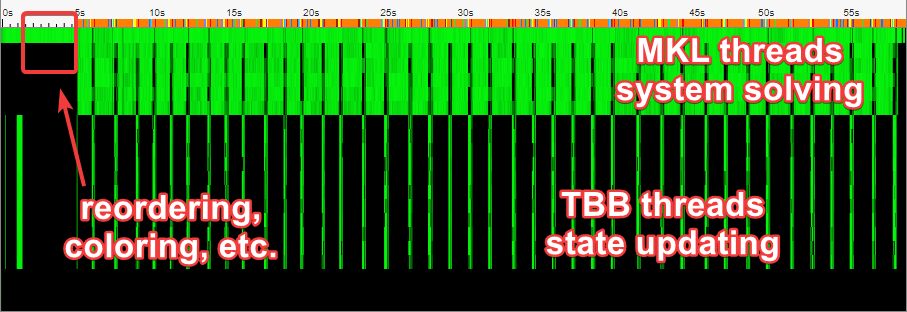
\includegraphics[width=.99\linewidth]{B1}
\end{figure}
\end{frame}
\begin{frame}{Benchmark}
manually override MKL defaults, not optimal but slightly faster
\begin{itemize}
\item \texttt{MKL\_DYNAMIC=FALSE}
\item \texttt{MKL\_NUM\_THREADS=12}
\item \SI{90}{\percent} CPU utilisation
\item 110 GFLOPS overall
\item 120 GFLOPS excluding initialisation
\end{itemize}
\begin{figure}[H]
\centering
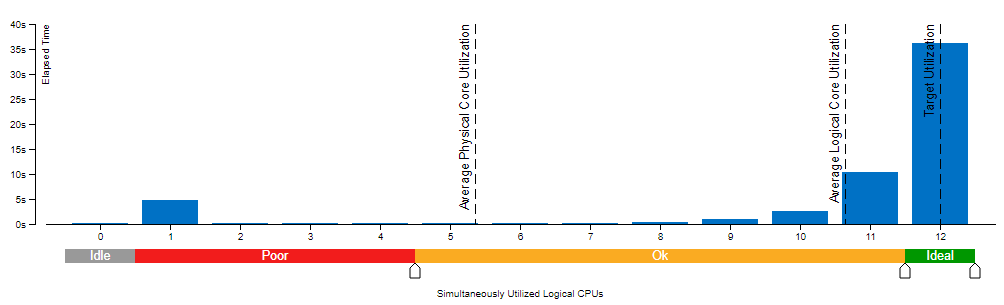
\includegraphics[width=.99\linewidth]{B3}
\end{figure}
\end{frame}
\begin{frame}{Benchmark}
about memory bounded (benchmark value \SI{25}{\giga\byte\per\second})
\begin{figure}[H]
\centering
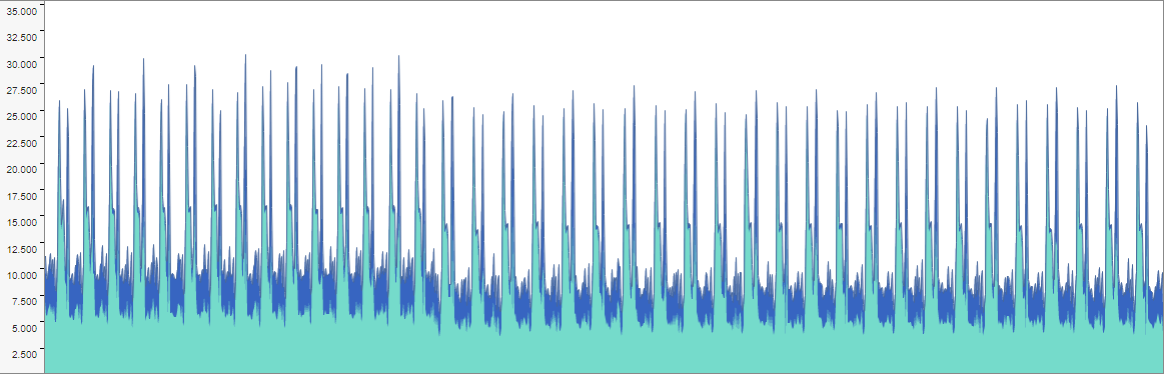
\includegraphics[width=.99\linewidth]{B4}
\end{figure}
\end{frame}
\begin{frame}{Benchmark}
\begin{figure}[H]
\centering
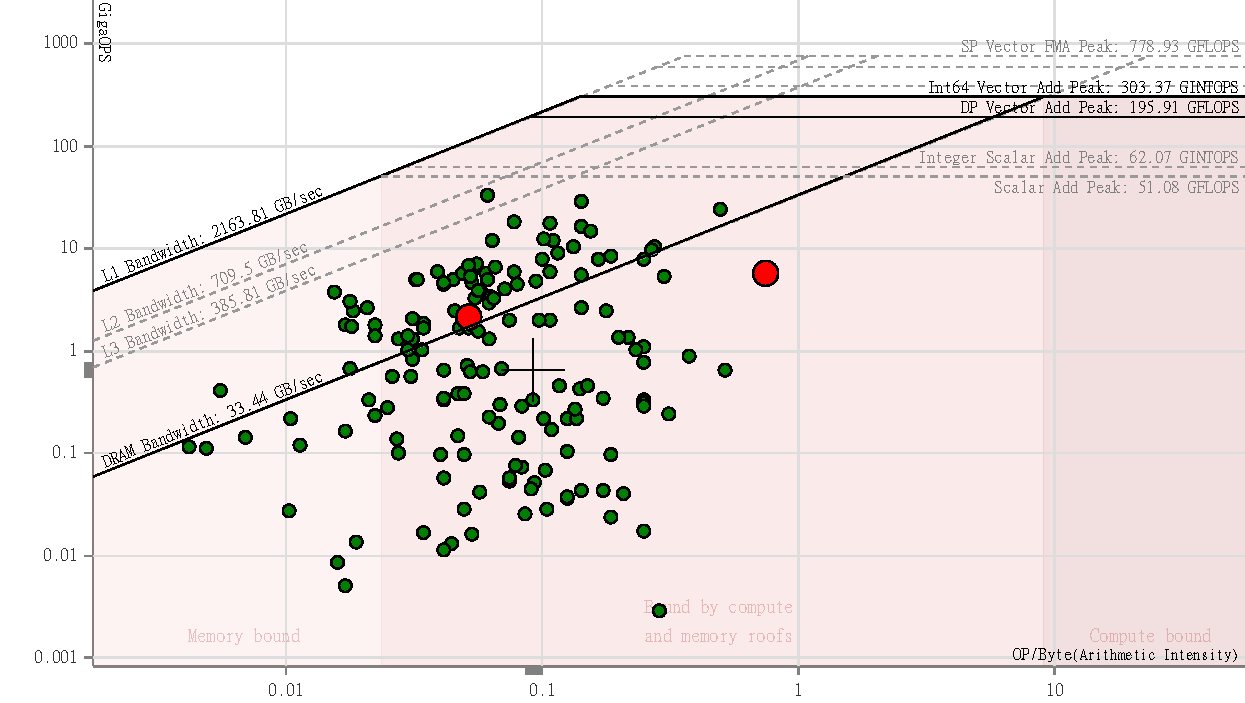
\includegraphics[width=.99\linewidth]{B5}
\end{figure}
\end{frame}
\begin{frame}{Summary}
Base parallelisation drivers: \texttt{std::execution}, \texttt{tbb}, \texttt{blas}, \texttt{lapack}, \texttt{scalapack}, \texttt{mpi}, \texttt{cuda}, etc.
\begin{itemize}
\item fully parallelised across all stages
\item task based parallelisation
\item relatively flat analysis logic
\item minimum data coupling/dependency
\item highly extensible
\end{itemize}

Future work: DPCPP (SYCL) unified shared memory (USM) based approach?
\end{frame}
%\begin{frame}{Some Thoughts}
%\begin{itemize}
%\item unified shared memory (USM) based OOP?
%\begin{itemize}
%\item local interface, remote data, remote computation
%\end{itemize}
%\end{itemize}
%\end{frame}
\begin{frame}[standout]
Thank you!
\end{frame}
\end{document}
